\aufgabe{LIME Superpixels}{
	
	Different methods for generating superpixels exist. 
	Here, the output of three different methods (one per column) is shown.
	
	\begin{figure}[H]
		\centering
		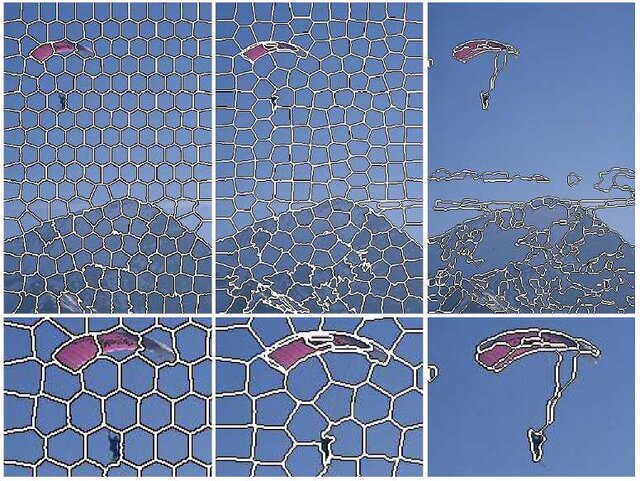
\includegraphics[width=.3\textwidth]{ex_tex/lime_superpixel_example}
		\caption{Examples of superpixel segmentation. Source: \href{https://doi.org/10.1016/j.imavis.2018.09.015}{MENDONCAOLIVEIRA2018}}
	\end{figure}
	
	\begin{enumerate}[a)]
		\item Each method is based on different underlying principles for generating superpixels. 
		Match the following descriptions to the corresponding images:
		
		\begin{enumerate}
			\item Superpixels align with meaningful object boundaries in the image.
			\item Superpixels have similar size and shape.
			\item Superpixels have similar size, the shape is specified by homogeneity in color/texture.
		\end{enumerate}
		
		\item How does the size of superpixels influence LIME explanations?
		Discuss the following questions in groups:
		
		\begin{enumerate}
			\item Does the number of features increase or decrease as the size of superpixels increases?
			\item Does it become easier or harder to localize specific influential regions when superpixel size increases?
		\end{enumerate}
		
	\end{enumerate}
}